\documentclass[a4paper, 11pt]{article}

\usepackage[utf8]{inputenc}
\usepackage{a4wide}
\usepackage{indentfirst}
\usepackage[normalem]{ulem}
\usepackage{setspace}
\usepackage{float}
\usepackage{graphicx}
\usepackage{subcaption}
\usepackage{hyperref}
\usepackage[capitalise]{cleveref}

\onehalfspacing

\begin{document}

\section{Privacy-preserving Data Publishing}

\textbf{1.1. One can identify 4 basic anonymization operations: generalization,
suppression, anatomization and perturbation. Anatomization consists on de-associating
QIDs and sensitive attributes. Explain what is the advantage and disadvantage of
anatomization?}

\vspace{\baselineskip}

Anatomization does not modify the quasi-identifier or the sensitive attribute, but
\uline{de-associates the relationship between the two}. In other words, this method
releases the data on $QID$ and the data on the sensitive attribute in two separate
tables: a quasi-identifier table ($QIT$) contains the $QID$ attributes, a sensitive table
($ST$) contains the sensitive attributes, and both $QIT$ and $ST$ have one common attribute,
$GroupID$. All records in the same group will have the same value on $GroupID$ in both
tables and, therefore, are linked to the sensitive values in the group in the exact
same way (\cref{fig:fig}).

\vspace{\baselineskip}

\begin{figure}[H]
\centering
\begin{subfigure}{.45\textwidth}
    \centering
    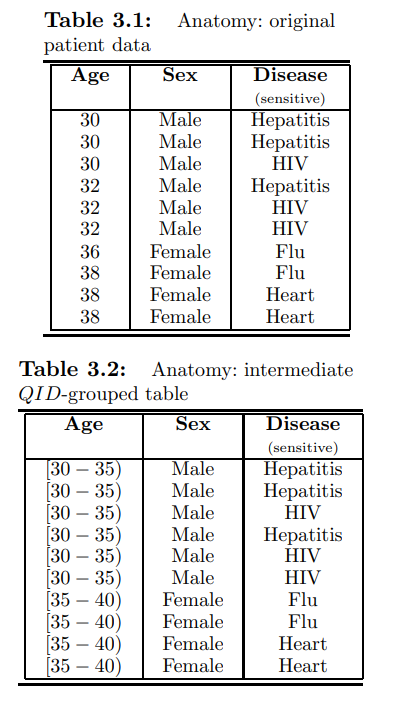
\includegraphics[width=\textwidth]{img/fig01.png}
\end{subfigure}%
\begin{subfigure}{.45\textwidth}
    \centering
    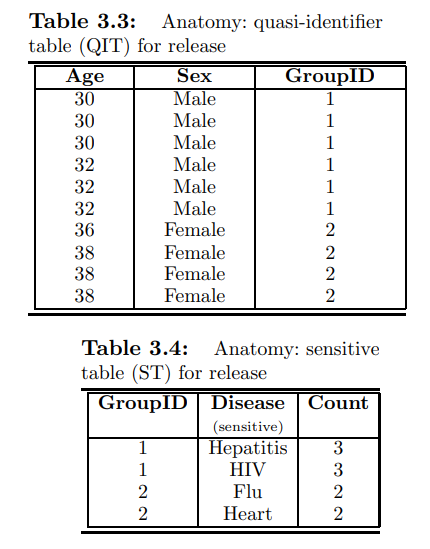
\includegraphics[width=\textwidth]{img/fig02.png}
\end{subfigure}
\caption{Anatomization}
\label{fig:fig}
\end{figure}

\vspace{2\baselineskip}

\textbf{Advantages}: The data in both $QIT$ and $ST$ are unmodified (unlike what
happens when we consider anonymization operations such as generalization or suppression).
The anatomized tables can more accurately answer aggregate queries involving domain
values of the $QID$ and sensitive attributes than the generalization approach.
The intuition is that in a generalized table domain values are lost and, without
additional knowledge, it is more difficult to answer a query about domain values.

\textbf{Disadvantages}: With the data published in two tables, it is unclear how
standard data mining tools (\textit{e.g.} classification and clustering data mining tools)
can be applied to the published data, and new tools and algorithms need to be designed.
Also, anatomization is not suitable for incremental data publishing. The generalization
approach does not suffer from the same problem because all attributes are released
in the same table.

\vspace{\baselineskip}

\textbf{1.2.} Differential privacy \underline{decreases}
 the risk of an individual/register joining or leaving the database.

\vspace{2\baselineskip}

\section{Secure Multiparty Computation and Privacy}

\textbf{2.1. In SMC two or more parties wish to jointly compute a function of their inputs
while preserving certain security properties, such as privacy, correctness and independence
of inputs. Considering the auction example, where users bid for a product, explain what
privacy means in this context.}

\vspace{\baselineskip}

Protocols for Secure Multiparty Computation (SMC) enable a set of parties to compute a
joint function of their private inputs while revealing nothing but the output. In
other words, the aim of secure multiparty computation is to enable parties to carry
out distributed computing tasks in a secure manner.

In this scenario, it is assumed that a protocol execution may be attacked by an external
entity, or even by a subset of the participating parties. The aim of this attack may be to
learn private information or cause the result of the computation to be incorrect. Thus,
two important requirements on any secure computation protocol are \textbf{privacy} and
\textbf{correctness}. The privacy requirement states that \uline{nothing should be
learned beyond what is absolutely necessary, \textit{i.e.}, parties should learn their
output and nothing else}. The correctness requirement states that \uline{each party
should receive its correct output. Therefore, the adversary must not be able to cause
the result of the computation to deviate from the function that the parties had set
out to compute}.

In the auction example, we consider a trading platform where parties provide offers
and bids, and are matched whenever an offer is greater than a bid. In such a scenario,
it can be beneficial to not reveal the parties’ actual offers and bids since this
information can be used by others in order to artificially raise prices.

In this scenario, the meaning of privacy and correctness is as follows:

\begin{itemize}
    \item \textbf{Privacy}: No party should learn anything more than its prescribed
    output. In particular, the only information that should be learned about other
    parties’ inputs is what can be derived from the output itself. In this case, the
    only bid revealed is that of the highest bidder, which makes it possible to infer
    that all other bids were lower than the winning bid. However, nothing else should
    be revealed about the losing bids.
    
    \item \textbf{Correctness}: Each party is guaranteed that the output that it
    receives is correct. In this case, this implies that the party with the highest
    bid is guaranteed to win, and no party including the auctioneer can influence this.
\end{itemize}

Other relevant properties of SMC include:

\begin{itemize}
    \item \textbf{Independence of Inputs}: Corrupted parties must choose their inputs
    independently of the honest parties’ inputs. This property is crucial in an 
    auction, where bids are kept secret and parties must fix their bids independently
    of others. Note that independence of inputs is not implied by privacy. For example,
    it may be possible to generate a higher bid, without knowing the value of the original
    one. Such an attack can actually be carried out on some encryption schemes (\textit{i.e.},
    given an encryption of \$100, it is possible to generate a valid encryption of \$101, without
    knowing the original encrypted value).
    
    \item \textbf{Guaranteed Output Delivery}: Corrupted parties should not be able to
    prevent honest parties from receiving their output. In other words, the adversary
    should not be able to disrupt the computation.
    
    \item \textbf{Fairness}: Corrupted parties should receive their outputs if and
    only if the honest parties also receive their outputs. The scenario where a
    corrupted party obtains output and an honest party does not should not be allowed
    to occur. Note that guaranteed output delivery implies fairness, but the converse
    is not necessarily true.  
\end{itemize}

\vspace{1.5\baselineskip}

\section{Authentication Protocols and Anonymous Authentication}

\paragraph{3.1.} Encryption and signing/authentication should be done with
\uline{two different public-key cryptography key pairs for each}.

\end{document}
